\documentclass[handout]{beamer}
%\documentclass{beamer}
\mode<presentation> {%
	\usetheme[]{Boadilla}
	\usecolortheme{orchid}
	\setbeamercovered{transparent}
	\setbeamersize{text margin left=0.7cm}
  \setbeamersize{text margin right=0.7cm}
  \setbeamertemplate{enumerate item}[square]
  \setbeamertemplate{enumerate subitem}[circle]
  \setbeamertemplate{enumerate subsubitem}[>]
  \setbeamertemplate{itemize item}[square]
  \setbeamertemplate{itemize subitem}[circle]
  \setbeamertemplate{itemize subsubitem}[>]
}

% \usepackage{bm}
\usepackage[utf8]{inputenc}
\usepackage[spanish]{babel}
% \usepackage[normalem]{ulem}
% \usepackage{times}
% \usepackage[T1]{fontenc}
\usepackage{graphicx}
% \usepackage{multirow}
% \usepackage{rotating}
% \usepackage{colortbl}
% \usepackage{verbatim}
\usepackage{hyperref}
\hypersetup{colorlinks=true,linkcolor=blue,urlcolor=blue}
\usepackage{tikz}
\usetikzlibrary{shapes.geometric, arrows, positioning}
\tikzstyle{block} = [rectangle, draw, text centered, rounded corners, minimum height=2em, align=center]
\tikzstyle{arrow} = [thick,->,>=stealth]

\definecolor{olivegreen}{rgb}{0.0,0.5,0.0}
\definecolor{general}{rgb}{0.9 0.9 1}%

\title[Procesamiento de Señales]{Muestreo y reconstrucción de señales \\ en el dominio del tiempo}
\author[Jesús Chacón] {%
	\textit{Ingeniería Electrónica de Comunicaciones}\\
	\vspace{0.6cm}
	\small Jesús Chacón Sombría%
}%\inst{1}

\institute[DACYA] {%\inst{1}%
	\footnotesize  Departamento de Arquitectura de Computadores y Automática\\
  Universidad Complutense de Madrid
}

\date[Muestreo y reconstrucción] % (optional)
{\footnotesize Curso 2024-2025}%{\today / Master}
\subject{Talks}

\pgfdeclareimage[height=0.75cm]{logo}{ucm}

\usepackage[absolute,overlay]{textpos}
\setlength{\TPHorizModule}{1mm}
\setlength{\TPVertModule}{1mm}
\newcommand{\MyLogo}{%
\begin{textblock}{14}(116.0,0.6)
  \pgfuseimage{logo}
\end{textblock}
}

\makeatletter
\numberwithin{section}{part}
\AtBeginPart{
\beamer@tocsectionnumber=0\relax
\frame{\partpage}
}
\makeatother

\begin{document}

\begin{frame}
  \titlepage
\end{frame}

\newcommand*\oldmacro{}%
\let\oldmacro\insertshorttitle%
\renewcommand*\insertshorttitle{%
 \MyLogo
  \oldmacro\hfill%
}

\AtBeginSection[]{}
\AtBeginSubsection[]{}

\section{Objetivos}
\section{Conversión analógico-digital y digital-analógico}
\section{Muestreo de señales continuas}
\subsection{Muestreo periódico}
\subsection{Teorema del muestreo}
  
  \begin{frame}
  \frametitle{Visión Continua y Discreta del Muestreo}
    \begin{itemize}
      \item Muestreo como una señal de tiempo continuo, o discreto:\\ 
      \[
        x_d(t) = \substack{\infty \\ \sum \\n=-\infty} x(t)\delta(t-nT_s)
        \quad\text{vs.}\quad
        x_d[n] = x_c(nT_s)
      \]
      
      \begin{itemize}
          \footnotesize
          \item La Transformada de Fourier de tiempo continuo (CFT) es: \\
          \[
          \begin{aligned}
          X_d(j\omega)&=\int_{-\infty}^{\infty}\left[\substack{\infty \\ \sum \\n=-\infty} x(t)\delta(t - nT_s)\right]e^{-j\omega t}dt\\
                      &=\substack{\infty \\ \sum \\n=-\infty} x(nT_s)e^{-j\omega T_s n}
          \end{aligned}
          \]
          \item La Transformada de Fourier de tiempo discreto (DTFT) es: \\
          \[
          X_d(\mathrm{e}^{j\Omega})=\substack{\infty \\ \sum \\n=-\infty} x(nT_s)e^{-j\Omega n}
          \]

        \end{itemize}
        \begin{alertblock}{Relación entre frecuencia continua $\omega$ y discreta $\Omega$}
            Comparando ambas expresiones, $X_d(j\omega)=X_d(\mathrm{e}^{j\Omega})$ si $\Omega=\omega T_s$.
        \end{alertblock}
    \end{itemize}    
  \end{frame}

  \begin{frame}
  \frametitle{Visión Continua y Discreta del Muestreo}
      \begin{alertblock}{Recordamos la relación entre el espectro de $X(j\omega)$ y $X_d(j\omega)$}
        \centering
        $X_d(\omega)=\frac{1}{T_s} \substack{\infty \\ \sum \\ -\infty} X(\omega - \frac{2\pi k}{T_s})$
      \end{alertblock}
      
      \begin{itemize}
        \item Si hacemos $\omega=\frac{\Omega}{T_s}$, entonces:
        \[
        X_d(\mathrm{e}^{j\Omega})= \frac{1}{T_s} \substack{\infty \\ \sum \\ -\infty} X(\frac{\Omega - 2\pi k}{T_s})
        \]
        \item Es decir, las frecuencias continuas $\omega\in(0, \pi/T_s)$ de la señal original se corresponden con las frecuencias discretas $\Omega\in(0, \pi)$.        
    \end{itemize}    
  \end{frame}

  \begin{frame}
  \frametitle{Visión Continua y Discreta del Muestreo}
      \begin{alertblock}{Recordamos la relación entre el espectro de $X(j\omega)$ y $X_d(j\omega)$}
        \centering
        $X_d(\omega)=\frac{1}{T_s} \substack{\infty \\ \sum \\ -\infty} X(\omega - \frac{2\pi k}{T_s})$
      \end{alertblock}
      
      \begin{itemize}
        \item El periodo de muestreo \emph{escala} el espectro de la señal original.
        \item En el límite $\omega_s=2\omega_m$ (\emph{Nyquist-Shannon}), el espectro de la señal discreta está \emph{completamente ocupado} por el de la señal continua.
        \item Si hacemos un sobremuestreo, p. ej. $\omega_s=4\:\omega_m$, estamos dejando un margen de frecuencias sin ocupar. 
    \end{itemize}    
  \end{frame}


  \begin{frame}\frametitle{Reconstrucción mediante interpolación}
    \begin{columns}[c]
      \begin{column}{4cm}
        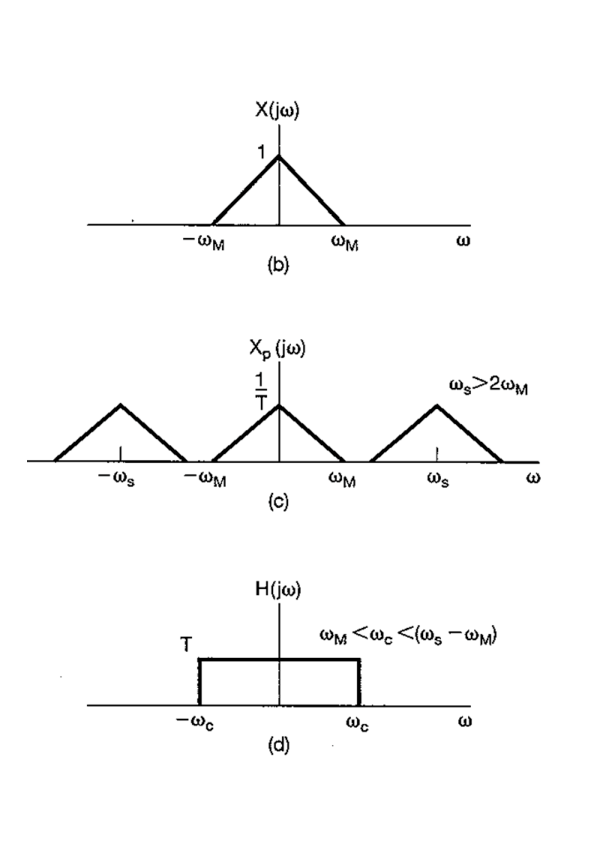
\includegraphics[width=5cm]{./Figures/RecIdeal}
      \end{column}
      \begin{column}{8cm}
      \begin{itemize}\footnotesize
        \item Retenedor orden cero: $H(j\omega)=e^{-j\frac{T_s\omega}{2}} T_s Sa(T_s\omega/2)$
        \item Retenedor orden uno: $H(j\omega)=T_s Sa^2(T_s \omega/2)$        
        \item Filtro ideal: $H(j\omega)=T_s \Pi(\frac{\omega}{\omega_s})$
      \end{itemize}
      
      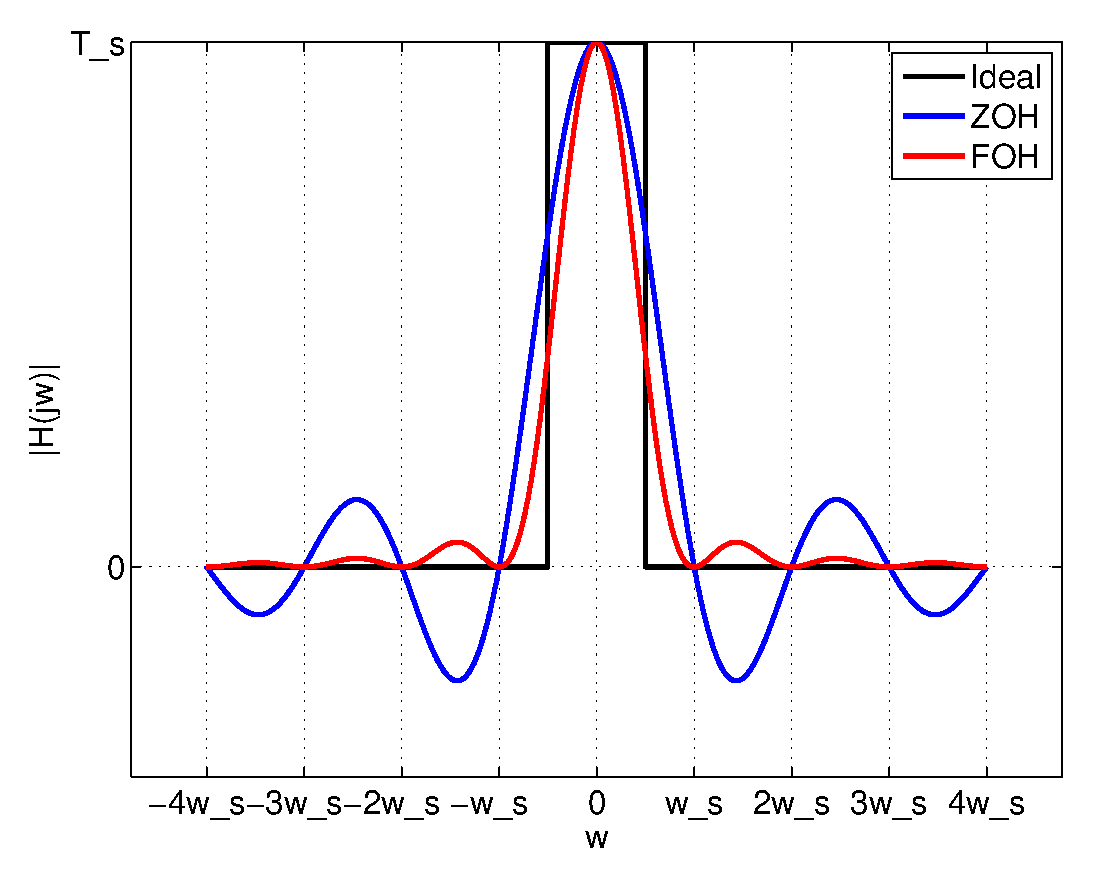
\includegraphics[width=4.5cm]{./Figures/Interpolacion.eps}      
      \end{column}
    \end{columns}
  \end{frame}
  
  
  \begin{frame}\frametitle{Retenedor de orden uno (FOH)}
    \footnotesize
  
    \begin{columns}[c]
      \hspace{-0.6cm}\begin{column}{8cm}
        \begin{itemize}
          \item Versión no causal:
          \begin{itemize}\footnotesize
            \item $h(t)=\Lambda(\frac{t}{T_s})$            
            \item $y(t)=\sum_{k=-\infty}^\infty x_c(kT)\Lambda(\frac{t-kT_s}{T_s})$
            \vspace{0.1cm}
            \item Es no causal porque:
            \begin{itemize}
              \item Durante el periodo $t \in (kT_s,(k\!+\!1)T_s)$:  $y(t)=x_c(kT)+\frac{x_c((k+1)T)-x_c(kT)}{T_s} (t-kT_s)$. Depende de un valor futuro. 
              \item Su h(t) toma valores no nulos en instantes previos a t=0.
            \end{itemize}
          \end{itemize}
          \item Versión causal:
          \begin{itemize}\footnotesize
            \item Durante el periodo $t \in (kT_s,(k\!+\!1)T_s)$: $y(t)=x_c(kT)+\frac{x_c(kT)-x_c((k-1)T)}{T_s} (t-kT_s)$
            \vspace{0.1cm}
            \item $h(t)=\Pi(\frac{t-T_s/2}{T_s})(1+\frac{t}{T_s})-\Pi(\frac{t-3T_s/2}{T_s})\frac{t-T_s}{T_s}$
            
            \vspace{0.1cm}
            \item Se puede calcular el espectro del filtro
          \end{itemize}
        \end{itemize}
      \end{column}
      \hspace{-0.6cm}\begin{column}{4cm}
        \only<1|handout:0>{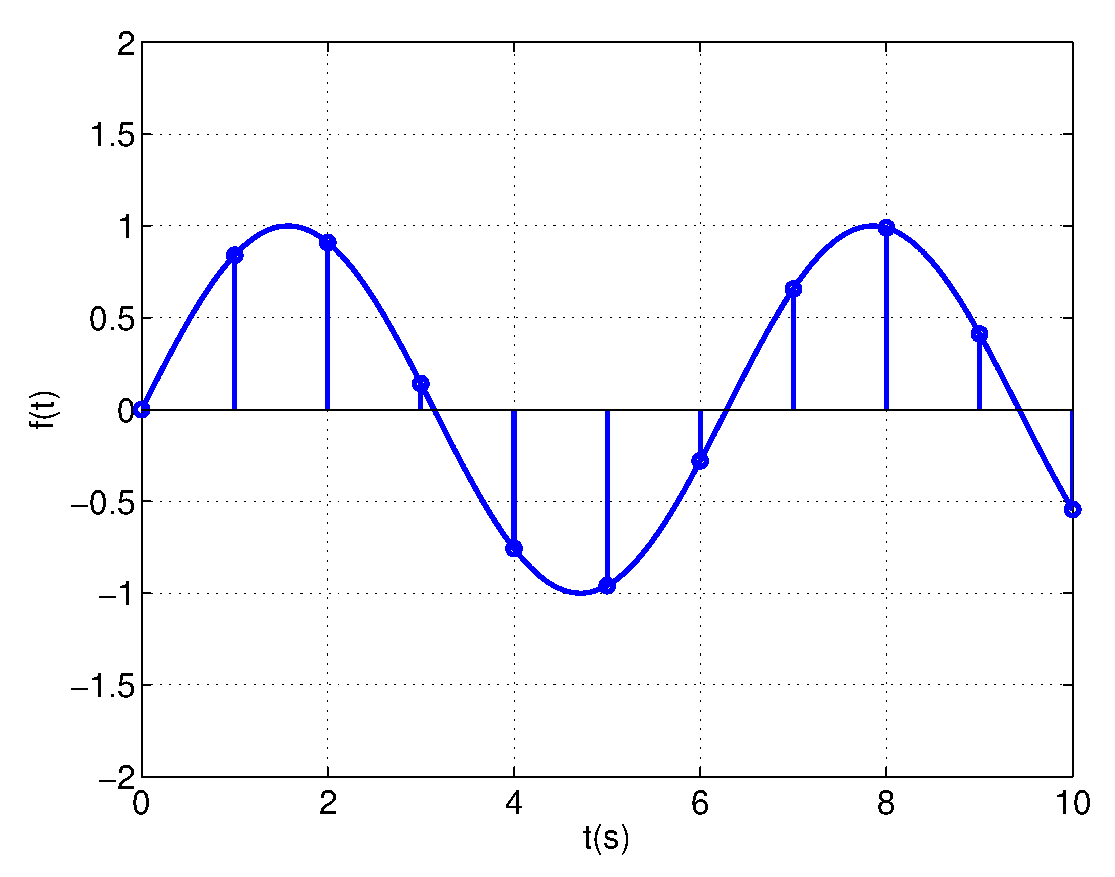
\includegraphics[width=4.5cm]{./Figures/FOHsTime0.eps}}\only<2-4|handout:0>{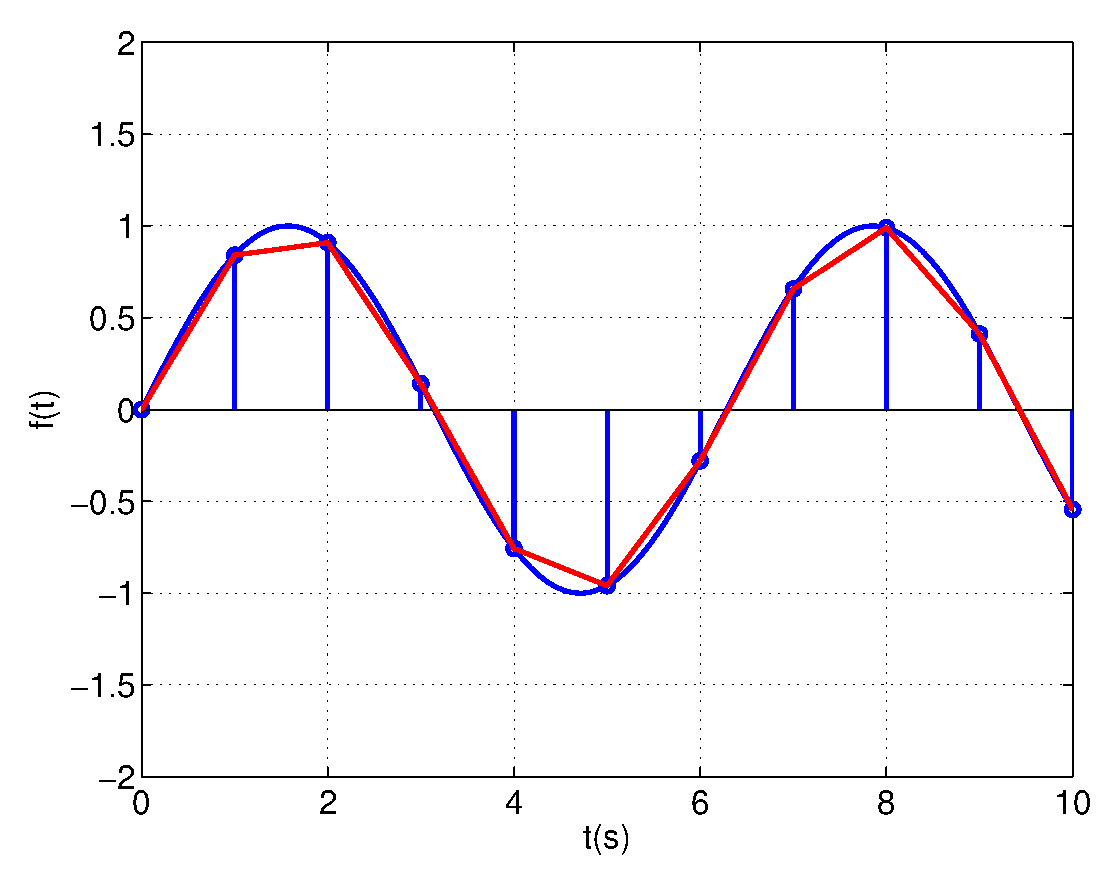
\includegraphics[width=4.5cm]{./Figures/FOHsTime1.eps}}\only<5->{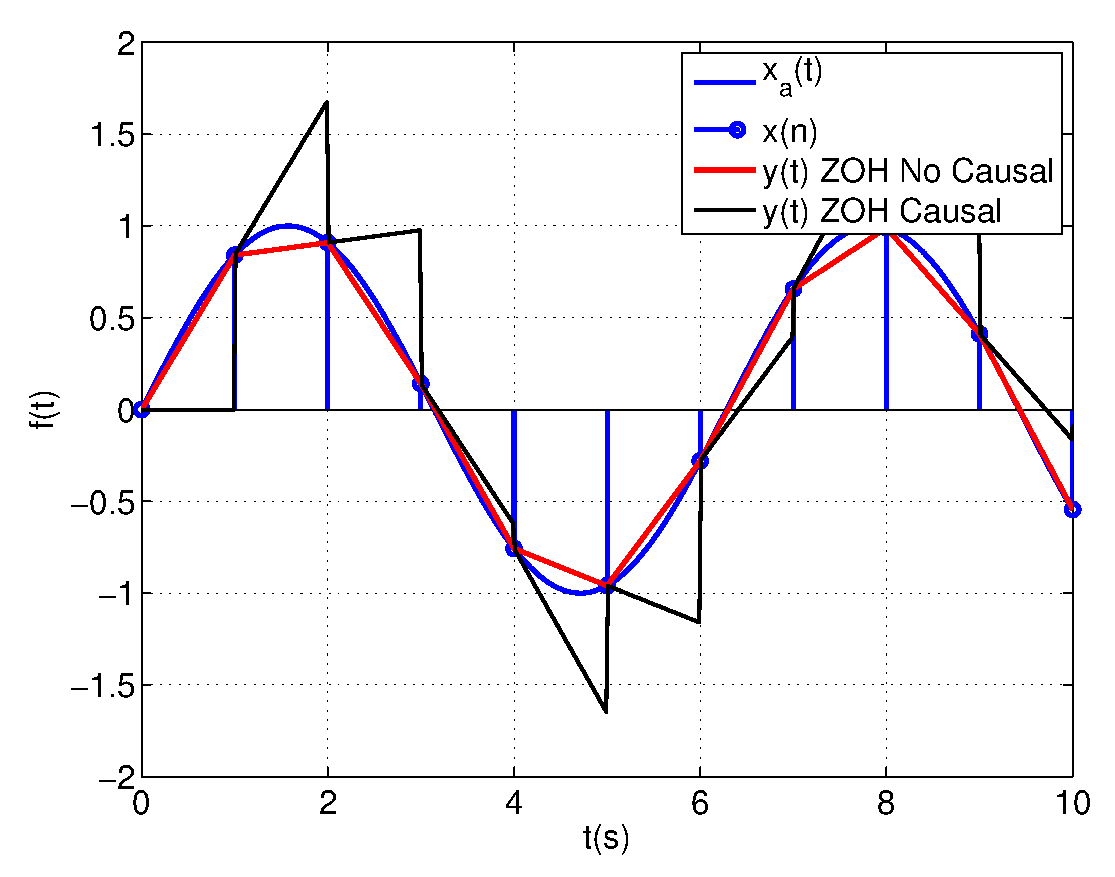
\includegraphics[width=4.5cm]{./Figures/FOHsTime.eps}}
        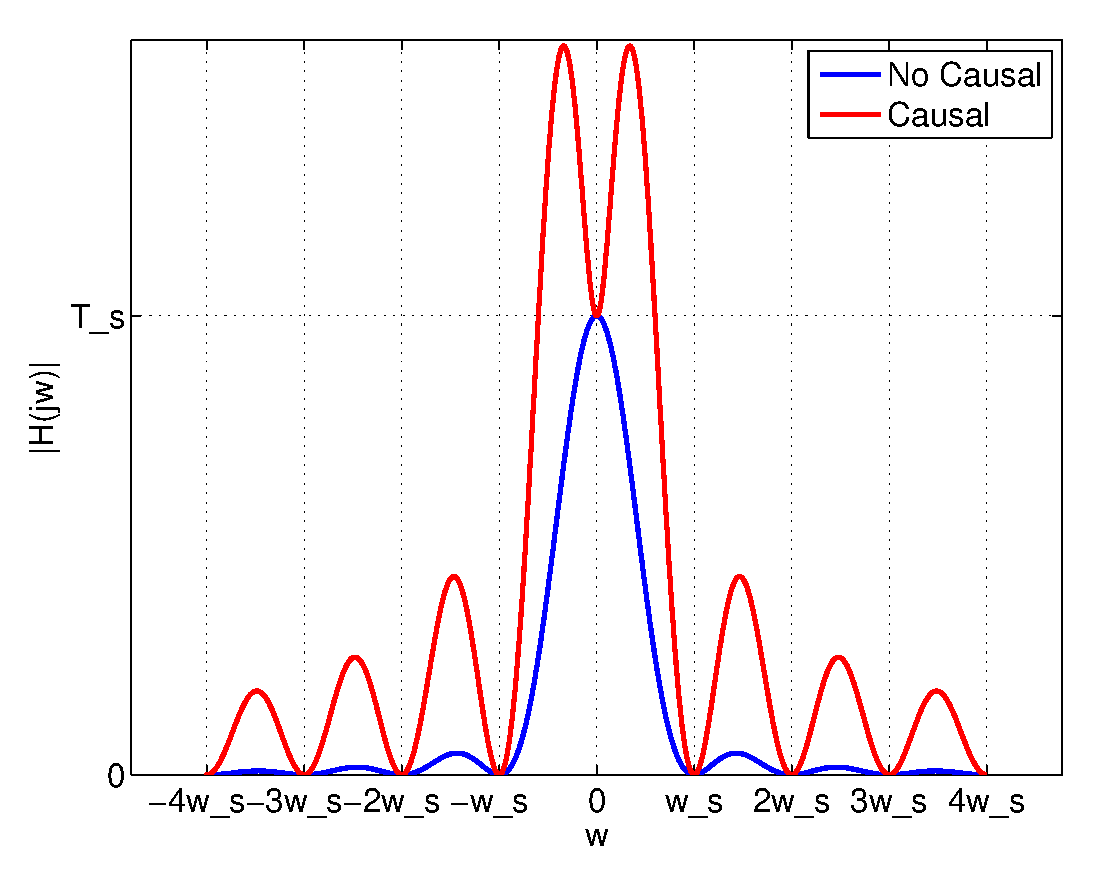
\includegraphics[width=4.5cm]{./Figures/FOHsFrec.eps}
      \end{column}
    \end{columns}
  \end{frame}

  \begin{frame}\frametitle{Conceptos importantes}
    \begin{itemize}
      \item \alert{Teorema del muestreo}
      \begin{itemize}
        \item Escalado y réplica
        \item $\omega_s>2\omega_m$ (para evitar solapamiento)
      \end{itemize}
      \item \alert{Reconstrucción}
      \begin{itemize}
        \item Filtro paso-bajo ideal (no realizable)
        \item Interpolación (FOH, retención de orden cero, etc.)
        \item En la práctica, reconstrucción no ideal, pero realizable.
      \end{itemize}
    \end{itemize}
  \end{frame}

\end{document}
